\documentclass{standalone}
\usepackage{tikz}
\usetikzlibrary{patterns, positioning}


\begin{document}
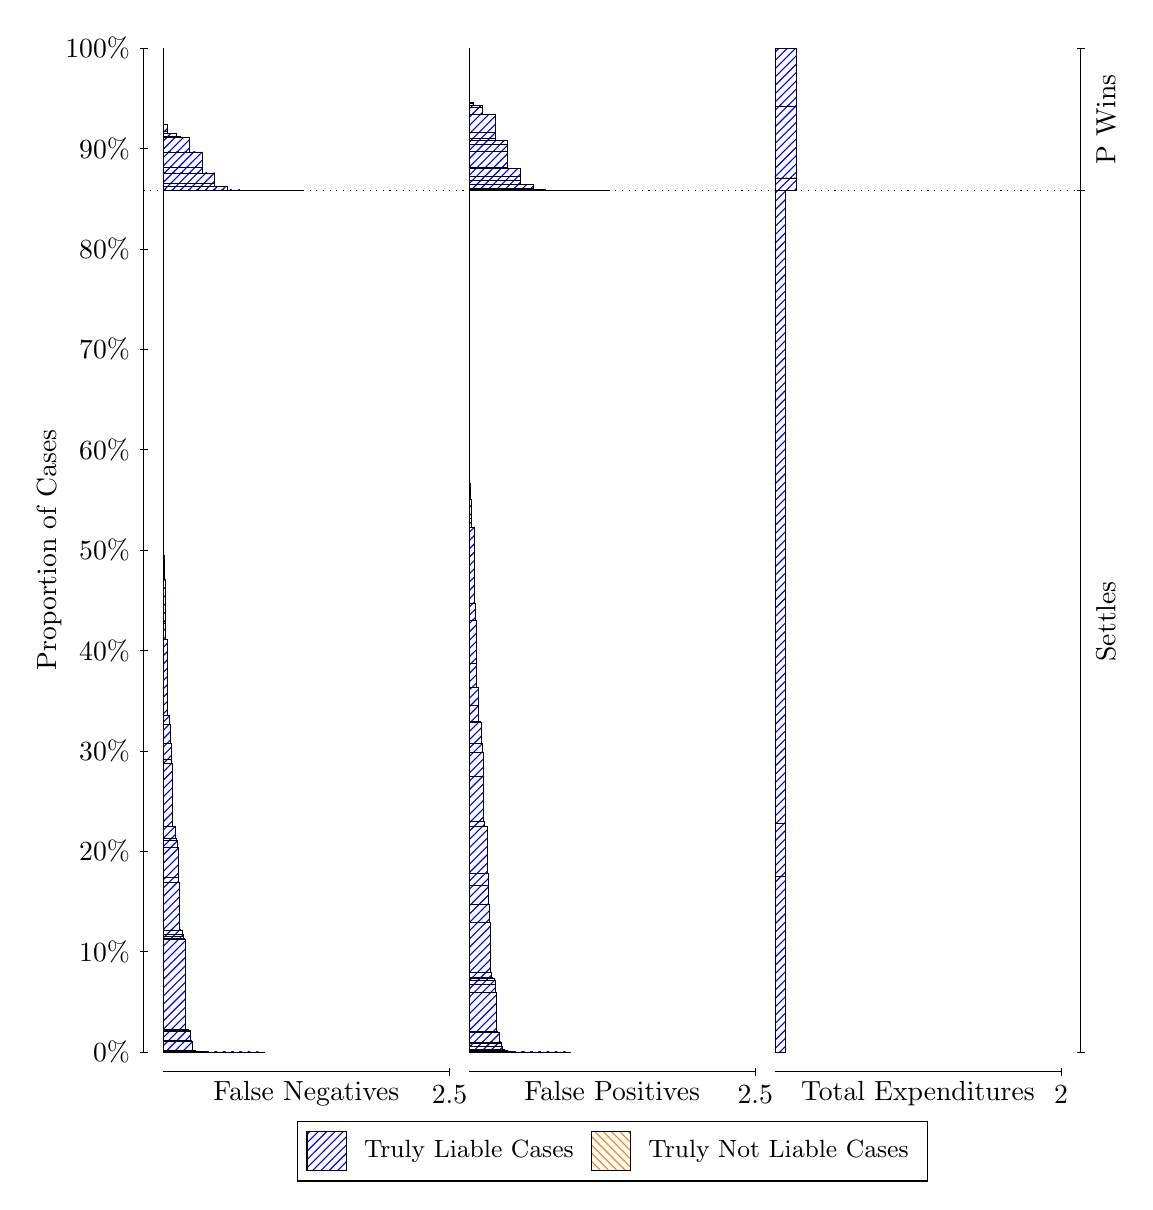
\begin{tikzpicture}
\draw[black, very thin] (1.5,1.75) -- (1.5,14.5);
\node[rotate=90, text=black, anchor=center] at (0.3, 8.125) {Proportion of Cases};
\draw[black, very thin] (1.45,1.75) -- (1.55,1.75);
\node[text=black, anchor=east] at (1.45, 1.75) {0\%};
\draw[black, very thin] (1.45,3.025) -- (1.55,3.025);
\node[text=black, anchor=east] at (1.45, 3.025) {10\%};
\draw[black, very thin] (1.45,4.3) -- (1.55,4.3);
\node[text=black, anchor=east] at (1.45, 4.3) {20\%};
\draw[black, very thin] (1.45,5.575) -- (1.55,5.575);
\node[text=black, anchor=east] at (1.45, 5.575) {30\%};
\draw[black, very thin] (1.45,6.85) -- (1.55,6.85);
\node[text=black, anchor=east] at (1.45, 6.85) {40\%};
\draw[black, very thin] (1.45,8.125) -- (1.55,8.125);
\node[text=black, anchor=east] at (1.45, 8.125) {50\%};
\draw[black, very thin] (1.45,9.4) -- (1.55,9.4);
\node[text=black, anchor=east] at (1.45, 9.4) {60\%};
\draw[black, very thin] (1.45,10.675) -- (1.55,10.675);
\node[text=black, anchor=east] at (1.45, 10.675) {70\%};
\draw[black, very thin] (1.45,11.95) -- (1.55,11.95);
\node[text=black, anchor=east] at (1.45, 11.95) {80\%};
\draw[black, very thin] (1.45,13.225) -- (1.55,13.225);
\node[text=black, anchor=east] at (1.45, 13.225) {90\%};
\draw[black, very thin] (1.45,14.5) -- (1.55,14.5);
\node[text=black, anchor=east] at (1.45, 14.5) {100\%};

\draw[black, very thin] (13.4,1.75) -- (13.4,14.5);
\draw[black, very thin] (13.35,1.75) -- (13.45,1.75);
\node[anchor=west] at (13.35, 1.75) {};
\draw[black, very thin] (13.35,12.688) -- (13.45,12.688);
\node[anchor=west] at (13.35, 12.688) {};
\draw[black, very thin] (13.35,14.5) -- (13.45,14.5);
\node[anchor=west] at (13.35, 14.5) {};

\draw[black, very thin, pattern color=blue, pattern=north east lines] (1.75,1.75) rectangle (3.0398,1.75);
\draw[black, very thin, pattern color=blue, pattern=north east lines] (1.75,1.75) rectangle (2.9672,1.75);
\draw[black, very thin, pattern color=blue, pattern=north east lines] (1.75,1.75) rectangle (2.8945,1.75);
\draw[black, very thin, pattern color=blue, pattern=north east lines] (1.75,1.75) rectangle (2.8784,1.75);
\draw[black, very thin, pattern color=blue, pattern=north east lines] (1.75,1.75) rectangle (2.8218,1.75);
\draw[black, very thin, pattern color=blue, pattern=north east lines] (1.75,1.75) rectangle (2.8057,1.75);
\draw[black, very thin, pattern color=blue, pattern=north east lines] (1.75,1.75) rectangle (2.7492,1.75);
\draw[black, very thin, pattern color=blue, pattern=north east lines] (1.75,1.75) rectangle (2.733,1.75);
\draw[black, very thin, pattern color=blue, pattern=north east lines] (1.75,1.75) rectangle (2.7169,1.75);
\draw[black, very thin, pattern color=blue, pattern=north east lines] (1.75,1.75) rectangle (2.6604,1.75);
\draw[black, very thin, pattern color=blue, pattern=north east lines] (1.75,1.75) rectangle (2.6442,1.75);
\draw[black, very thin, pattern color=blue, pattern=north east lines] (1.75,1.75) rectangle (2.6038,1.75);
\draw[black, very thin, pattern color=blue, pattern=north east lines] (1.75,1.75) rectangle (2.5877,1.75);
\draw[black, very thin, pattern color=blue, pattern=north east lines] (1.75,1.75) rectangle (2.5715,1.75);
\draw[black, very thin, pattern color=blue, pattern=north east lines] (1.75,1.75) rectangle (2.5554,1.75);
\draw[black, very thin, pattern color=blue, pattern=north east lines] (1.75,1.75) rectangle (2.5312,1.75);
\draw[black, very thin, pattern color=blue, pattern=north east lines] (1.75,1.75) rectangle (2.4989,1.75);
\draw[black, very thin, pattern color=blue, pattern=north east lines] (1.75,1.75) rectangle (2.4827,1.75);
\draw[black, very thin, pattern color=blue, pattern=north east lines] (1.75,1.75) rectangle (2.4585,1.75);
\draw[black, very thin, pattern color=blue, pattern=north east lines] (1.75,1.75) rectangle (2.4424,1.7501);
\draw[black, very thin, pattern color=blue, pattern=north east lines] (1.75,1.7501) rectangle (2.4262,1.7501);
\draw[black, very thin, pattern color=blue, pattern=north east lines] (1.75,1.7501) rectangle (2.4101,1.7501);
\draw[black, very thin, pattern color=blue, pattern=north east lines] (1.75,1.7501) rectangle (2.3939,1.7501);
\draw[black, very thin, pattern color=blue, pattern=north east lines] (1.75,1.7501) rectangle (2.3858,1.7501);
\draw[black, very thin, pattern color=blue, pattern=north east lines] (1.75,1.7501) rectangle (2.3697,1.7501);
\draw[black, very thin, pattern color=blue, pattern=north east lines] (1.75,1.7501) rectangle (2.3374,1.7501);
\draw[black, very thin, pattern color=blue, pattern=north east lines] (1.75,1.7501) rectangle (2.3212,1.7501);
\draw[black, very thin, pattern color=blue, pattern=north east lines] (1.75,1.7501) rectangle (2.3132,1.7505);
\draw[black, very thin, pattern color=blue, pattern=north east lines] (1.75,1.7505) rectangle (2.297,1.7505);
\draw[black, very thin, pattern color=blue, pattern=north east lines] (1.75,1.7505) rectangle (2.2809,1.7562);
\draw[black, very thin, pattern color=blue, pattern=north east lines] (1.75,1.7562) rectangle (2.2647,1.7563);
\draw[black, very thin, pattern color=blue, pattern=north east lines] (1.75,1.7563) rectangle (2.2486,1.7564);
\draw[black, very thin, pattern color=blue, pattern=north east lines] (1.75,1.7564) rectangle (2.2324,1.7564);
\draw[black, very thin, pattern color=blue, pattern=north east lines] (1.75,1.7564) rectangle (2.2244,1.7569);
\draw[black, very thin, pattern color=blue, pattern=north east lines] (1.75,1.7569) rectangle (2.2082,1.7569);
\draw[black, very thin, pattern color=blue, pattern=north east lines] (1.75,1.7569) rectangle (2.1759,1.7571);
\draw[black, very thin, pattern color=blue, pattern=north east lines] (1.75,1.7571) rectangle (2.1678,1.7582);
\draw[black, very thin, pattern color=blue, pattern=north east lines] (1.75,1.7582) rectangle (2.1598,1.7587);
\draw[black, very thin, pattern color=blue, pattern=north east lines] (1.75,1.7587) rectangle (2.1517,1.7666);
\draw[black, very thin, pattern color=blue, pattern=north east lines] (1.75,1.7666) rectangle (2.1355,1.7666);
\draw[black, very thin, pattern color=blue, pattern=north east lines] (1.75,1.7666) rectangle (2.1194,1.8879);
\draw[black, very thin, pattern color=blue, pattern=north east lines] (1.75,1.8879) rectangle (2.1032,1.8931);
\draw[black, very thin, pattern color=blue, pattern=north east lines] (1.75,1.8931) rectangle (2.0952,2.0147);
\draw[black, very thin, pattern color=blue, pattern=north east lines] (1.75,2.0147) rectangle (2.0871,2.0199);
\draw[black, very thin, pattern color=blue, pattern=north east lines] (1.75,2.0199) rectangle (2.0709,2.0204);
\draw[black, very thin, pattern color=blue, pattern=north east lines] (1.75,2.0204) rectangle (2.0629,2.0412);
\draw[black, very thin, pattern color=blue, pattern=north east lines] (1.75,2.0412) rectangle (2.0467,2.0414);
\draw[black, very thin, pattern color=blue, pattern=north east lines] (1.75,2.0414) rectangle (2.0225,3.1828);
\draw[black, very thin, pattern color=blue, pattern=north east lines] (1.75,3.1828) rectangle (2.0144,3.1897);
\draw[black, very thin, pattern color=blue, pattern=north east lines] (1.75,3.1897) rectangle (2.0064,3.2165);
\draw[black, very thin, pattern color=blue, pattern=north east lines] (1.75,3.2165) rectangle (1.9983,3.2422);
\draw[black, very thin, pattern color=blue, pattern=north east lines] (1.75,3.2422) rectangle (1.9902,3.3013);
\draw[black, very thin, pattern color=blue, pattern=north east lines] (1.75,3.3013) rectangle (1.9741,3.3014);
\draw[black, very thin, pattern color=blue, pattern=north east lines] (1.75,3.3014) rectangle (1.9579,3.9001);
\draw[black, very thin, pattern color=blue, pattern=north east lines] (1.75,3.9001) rectangle (1.9418,3.9671);
\draw[black, very thin, pattern color=blue, pattern=north east lines] (1.75,3.9671) rectangle (1.9337,4.3506);
\draw[black, very thin, pattern color=blue, pattern=north east lines] (1.75,4.3506) rectangle (1.9256,4.4438);
\draw[black, very thin, pattern color=blue, pattern=north east lines] (1.75,4.4438) rectangle (1.9095,4.4675);
\draw[black, very thin, pattern color=blue, pattern=north east lines] (1.75,4.4675) rectangle (1.9014,4.618);
\draw[black, very thin, pattern color=blue, pattern=north east lines] (1.75,4.618) rectangle (1.8852,4.6199);
\draw[black, very thin, pattern color=blue, pattern=north east lines] (1.75,4.6199) rectangle (1.861,5.4123);
\draw[black, very thin, pattern color=blue, pattern=north east lines] (1.75,5.4123) rectangle (1.8529,5.4705);
\draw[black, very thin, pattern color=blue, pattern=north east lines] (1.75,5.4705) rectangle (1.8449,5.6654);
\draw[black, very thin, pattern color=blue, pattern=north east lines] (1.75,5.6654) rectangle (1.8368,5.9092);
\draw[black, very thin, pattern color=blue, pattern=north east lines] (1.75,5.9092) rectangle (1.8287,6.0305);
\draw[black, very thin, pattern color=blue, pattern=north east lines] (1.75,6.0305) rectangle (1.8126,6.031);
\draw[black, very thin, pattern color=blue, pattern=north east lines] (1.75,6.031) rectangle (1.7964,6.9885);
\draw[black, very thin, pattern color=blue, pattern=north east lines] (1.75,6.9885) rectangle (1.7803,7.1998);
\draw[black, very thin, pattern color=blue, pattern=north east lines] (1.75,7.1998) rectangle (1.7722,7.7524);
\draw[black, very thin, pattern color=blue, pattern=north east lines] (1.75,7.7524) rectangle (1.7641,8.0612);
\draw[black, very thin, pattern color=orange, pattern=north west lines] (1.75,8.0612) rectangle (1.75,8.0612);
\draw[black, very thin, pattern color=blue, pattern=north east lines] (1.75,8.0612) rectangle (1.75,12.688);
\draw[black, very thin, pattern color=blue, pattern=north east lines] (1.75,12.688) rectangle (3.5303,12.688);
\draw[black, very thin, pattern color=blue, pattern=north east lines] (1.75,12.688) rectangle (3.3689,12.688);
\draw[black, very thin, pattern color=blue, pattern=north east lines] (1.75,12.688) rectangle (3.2074,12.688);
\draw[black, very thin, pattern color=blue, pattern=north east lines] (1.75,12.688) rectangle (3.0459,12.689);
\draw[black, very thin, pattern color=blue, pattern=north east lines] (1.75,12.689) rectangle (2.8844,12.689);
\draw[black, very thin, pattern color=blue, pattern=north east lines] (1.75,12.689) rectangle (2.8844,12.69);
\draw[black, very thin, pattern color=blue, pattern=north east lines] (1.75,12.69) rectangle (2.7714,12.69);
\draw[black, very thin, pattern color=blue, pattern=north east lines] (1.75,12.69) rectangle (2.7229,12.694);
\draw[black, very thin, pattern color=blue, pattern=north east lines] (1.75,12.694) rectangle (2.7229,12.698);
\draw[black, very thin, pattern color=blue, pattern=north east lines] (1.75,12.698) rectangle (2.6099,12.698);
\draw[black, very thin, pattern color=blue, pattern=north east lines] (1.75,12.698) rectangle (2.6099,12.698);
\draw[black, very thin, pattern color=blue, pattern=north east lines] (1.75,12.698) rectangle (2.5614,12.745);
\draw[black, very thin, pattern color=blue, pattern=north east lines] (1.75,12.745) rectangle (2.5614,12.747);
\draw[black, very thin, pattern color=blue, pattern=north east lines] (1.75,12.747) rectangle (2.4484,12.747);
\draw[black, very thin, pattern color=blue, pattern=north east lines] (1.75,12.747) rectangle (2.4484,12.747);
\draw[black, very thin, pattern color=blue, pattern=north east lines] (1.75,12.747) rectangle (2.4484,12.747);
\draw[black, very thin, pattern color=blue, pattern=north east lines] (1.75,12.747) rectangle (2.4,12.777);
\draw[black, very thin, pattern color=blue, pattern=north east lines] (1.75,12.777) rectangle (2.4,12.913);
\draw[black, very thin, pattern color=blue, pattern=north east lines] (1.75,12.913) rectangle (2.2869,12.913);
\draw[black, very thin, pattern color=blue, pattern=north east lines] (1.75,12.913) rectangle (2.2869,12.913);
\draw[black, very thin, pattern color=blue, pattern=north east lines] (1.75,12.913) rectangle (2.2385,12.991);
\draw[black, very thin, pattern color=blue, pattern=north east lines] (1.75,12.991) rectangle (2.2385,13.175);
\draw[black, very thin, pattern color=blue, pattern=north east lines] (1.75,13.175) rectangle (2.2385,13.181);
\draw[black, very thin, pattern color=blue, pattern=north east lines] (1.75,13.181) rectangle (2.1254,13.181);
\draw[black, very thin, pattern color=blue, pattern=north east lines] (1.75,13.181) rectangle (2.1254,13.181);
\draw[black, very thin, pattern color=blue, pattern=north east lines] (1.75,13.181) rectangle (2.1254,13.182);
\draw[black, very thin, pattern color=blue, pattern=north east lines] (1.75,13.182) rectangle (2.077,13.363);
\draw[black, very thin, pattern color=blue, pattern=north east lines] (1.75,13.363) rectangle (1.964,13.376);
\draw[black, very thin, pattern color=blue, pattern=north east lines] (1.75,13.376) rectangle (1.964,13.376);
\draw[black, very thin, pattern color=blue, pattern=north east lines] (1.75,13.376) rectangle (1.9155,13.377);
\draw[black, very thin, pattern color=blue, pattern=north east lines] (1.75,13.377) rectangle (1.9155,13.418);
\draw[black, very thin, pattern color=blue, pattern=north east lines] (1.75,13.418) rectangle (1.9155,13.418);
\draw[black, very thin, pattern color=blue, pattern=north east lines] (1.75,13.418) rectangle (1.8025,13.441);
\draw[black, very thin, pattern color=blue, pattern=north east lines] (1.75,13.441) rectangle (1.8025,13.533);
\draw[black, very thin, pattern color=blue, pattern=north east lines] (1.75,13.533) rectangle (1.754,13.534);
\draw[black, very thin, pattern color=blue, pattern=north east lines] (1.75,13.534) rectangle (1.754,13.534);
\draw[black, very thin, pattern color=orange, pattern=north west lines] (1.75,13.534) rectangle (1.75,13.534);
\draw[black, very thin, pattern color=blue, pattern=north east lines] (1.75,13.534) rectangle (1.75,14.5);
\draw[black, very thin, pattern color=orange, pattern=north west lines] (5.6333,1.75) rectangle (6.9232,1.75);
\draw[black, very thin, pattern color=blue, pattern=north east lines] (5.6333,1.75) rectangle (6.9232,1.75);
\draw[black, very thin, pattern color=orange, pattern=north west lines] (5.6333,1.75) rectangle (6.8505,1.75);
\draw[black, very thin, pattern color=blue, pattern=north east lines] (5.6333,1.75) rectangle (6.8505,1.75);
\draw[black, very thin, pattern color=orange, pattern=north west lines] (5.6333,1.75) rectangle (6.7778,1.75);
\draw[black, very thin, pattern color=blue, pattern=north east lines] (5.6333,1.75) rectangle (6.7778,1.75);
\draw[black, very thin, pattern color=blue, pattern=north east lines] (5.6333,1.75) rectangle (6.7617,1.75);
\draw[black, very thin, pattern color=blue, pattern=north east lines] (5.6333,1.75) rectangle (6.689,1.75);
\draw[black, very thin, pattern color=orange, pattern=north west lines] (5.6333,1.75) rectangle (6.6325,1.75);
\draw[black, very thin, pattern color=blue, pattern=north east lines] (5.6333,1.75) rectangle (6.6325,1.75);
\draw[black, very thin, pattern color=blue, pattern=north east lines] (5.6333,1.75) rectangle (6.6164,1.75);
\draw[black, very thin, pattern color=blue, pattern=north east lines] (5.6333,1.75) rectangle (6.6002,1.75);
\draw[black, very thin, pattern color=orange, pattern=north west lines] (5.6333,1.75) rectangle (6.5598,1.75);
\draw[black, very thin, pattern color=blue, pattern=north east lines] (5.6333,1.75) rectangle (6.5598,1.75);
\draw[black, very thin, pattern color=blue, pattern=north east lines] (5.6333,1.75) rectangle (6.5275,1.75);
\draw[black, very thin, pattern color=orange, pattern=north west lines] (5.6333,1.75) rectangle (6.4872,1.75);
\draw[black, very thin, pattern color=blue, pattern=north east lines] (5.6333,1.75) rectangle (6.4872,1.75);
\draw[black, very thin, pattern color=blue, pattern=north east lines] (5.6333,1.75) rectangle (6.471,1.75);
\draw[black, very thin, pattern color=blue, pattern=north east lines] (5.6333,1.75) rectangle (6.4549,1.75);
\draw[black, very thin, pattern color=blue, pattern=north east lines] (5.6333,1.75) rectangle (6.4387,1.75);
\draw[black, very thin, pattern color=orange, pattern=north west lines] (5.6333,1.75) rectangle (6.4145,1.75);
\draw[black, very thin, pattern color=blue, pattern=north east lines] (5.6333,1.75) rectangle (6.4145,1.75);
\draw[black, very thin, pattern color=blue, pattern=north east lines] (5.6333,1.75) rectangle (6.3984,1.75);
\draw[black, very thin, pattern color=blue, pattern=north east lines] (5.6333,1.75) rectangle (6.3661,1.75);
\draw[black, very thin, pattern color=orange, pattern=north west lines] (5.6333,1.75) rectangle (6.3418,1.75);
\draw[black, very thin, pattern color=blue, pattern=north east lines] (5.6333,1.75) rectangle (6.3418,1.7501);
\draw[black, very thin, pattern color=blue, pattern=north east lines] (5.6333,1.7501) rectangle (6.3257,1.7501);
\draw[black, very thin, pattern color=blue, pattern=north east lines] (5.6333,1.7501) rectangle (6.3095,1.7501);
\draw[black, very thin, pattern color=blue, pattern=north east lines] (5.6333,1.7501) rectangle (6.2934,1.7502);
\draw[black, very thin, pattern color=blue, pattern=north east lines] (5.6333,1.7502) rectangle (6.2772,1.7502);
\draw[black, very thin, pattern color=blue, pattern=north east lines] (5.6333,1.7502) rectangle (6.253,1.7502);
\draw[black, very thin, pattern color=blue, pattern=north east lines] (5.6333,1.7502) rectangle (6.2369,1.7502);
\draw[black, very thin, pattern color=blue, pattern=north east lines] (5.6333,1.7502) rectangle (6.2046,1.7508);
\draw[black, very thin, pattern color=orange, pattern=north west lines] (5.6333,1.7508) rectangle (6.1965,1.7508);
\draw[black, very thin, pattern color=blue, pattern=north east lines] (5.6333,1.7508) rectangle (6.1965,1.7518);
\draw[black, very thin, pattern color=blue, pattern=north east lines] (5.6333,1.7518) rectangle (6.1804,1.7583);
\draw[black, very thin, pattern color=blue, pattern=north east lines] (5.6333,1.7583) rectangle (6.1642,1.7583);
\draw[black, very thin, pattern color=blue, pattern=north east lines] (5.6333,1.7583) rectangle (6.1481,1.7585);
\draw[black, very thin, pattern color=blue, pattern=north east lines] (5.6333,1.7585) rectangle (6.1319,1.7637);
\draw[black, very thin, pattern color=orange, pattern=north west lines] (5.6333,1.7637) rectangle (6.1238,1.7637);
\draw[black, very thin, pattern color=blue, pattern=north east lines] (5.6333,1.7637) rectangle (6.1238,1.774);
\draw[black, very thin, pattern color=blue, pattern=north east lines] (5.6333,1.774) rectangle (6.1158,1.7745);
\draw[black, very thin, pattern color=blue, pattern=north east lines] (5.6333,1.7745) rectangle (6.0915,1.7747);
\draw[black, very thin, pattern color=blue, pattern=north east lines] (5.6333,1.7747) rectangle (6.0754,1.7799);
\draw[black, very thin, pattern color=orange, pattern=north west lines] (5.6333,1.7799) rectangle (6.0512,1.7799);
\draw[black, very thin, pattern color=blue, pattern=north east lines] (5.6333,1.7799) rectangle (6.0512,1.8287);
\draw[black, very thin, pattern color=blue, pattern=north east lines] (5.6333,1.8287) rectangle (6.0431,1.8545);
\draw[black, very thin, pattern color=blue, pattern=north east lines] (5.6333,1.8545) rectangle (6.035,1.8781);
\draw[black, very thin, pattern color=blue, pattern=north east lines] (5.6333,1.8781) rectangle (6.0189,2.0009);
\draw[black, very thin, pattern color=blue, pattern=north east lines] (5.6333,2.0009) rectangle (6.0027,2.001);
\draw[black, very thin, pattern color=blue, pattern=north east lines] (5.6333,2.001) rectangle (5.9866,2.0079);
\draw[black, very thin, pattern color=orange, pattern=north west lines] (5.6333,2.0079) rectangle (5.9785,2.0079);
\draw[black, very thin, pattern color=blue, pattern=north east lines] (5.6333,2.0079) rectangle (5.9785,2.5115);
\draw[black, very thin, pattern color=blue, pattern=north east lines] (5.6333,2.5115) rectangle (5.9704,2.6046);
\draw[black, very thin, pattern color=blue, pattern=north east lines] (5.6333,2.6046) rectangle (5.9624,2.6657);
\draw[black, very thin, pattern color=blue, pattern=north east lines] (5.6333,2.6657) rectangle (5.9543,2.6919);
\draw[black, very thin, pattern color=blue, pattern=north east lines] (5.6333,2.6919) rectangle (5.9301,2.6938);
\draw[black, very thin, pattern color=blue, pattern=north east lines] (5.6333,2.6938) rectangle (5.9139,2.7607);
\draw[black, very thin, pattern color=orange, pattern=north west lines] (5.6333,2.7607) rectangle (5.9058,2.7607);
\draw[black, very thin, pattern color=blue, pattern=north east lines] (5.6333,2.7607) rectangle (5.9058,3.3986);
\draw[black, very thin, pattern color=blue, pattern=north east lines] (5.6333,3.3986) rectangle (5.8897,3.6197);
\draw[black, very thin, pattern color=blue, pattern=north east lines] (5.6333,3.6197) rectangle (5.8816,3.8653);
\draw[black, very thin, pattern color=blue, pattern=north east lines] (5.6333,3.8653) rectangle (5.8735,4.0177);
\draw[black, very thin, pattern color=blue, pattern=north east lines] (5.6333,4.0177) rectangle (5.8574,4.6172);
\draw[black, very thin, pattern color=blue, pattern=north east lines] (5.6333,4.6172) rectangle (5.8412,4.6177);
\draw[black, very thin, pattern color=blue, pattern=north east lines] (5.6333,4.6177) rectangle (5.8251,4.6761);
\draw[black, very thin, pattern color=blue, pattern=north east lines] (5.6333,4.6761) rectangle (5.817,5.2473);
\draw[black, very thin, pattern color=blue, pattern=north east lines] (5.6333,5.2473) rectangle (5.8089,5.5525);
\draw[black, very thin, pattern color=blue, pattern=north east lines] (5.6333,5.5525) rectangle (5.8009,5.6728);
\draw[black, very thin, pattern color=blue, pattern=north east lines] (5.6333,5.6728) rectangle (5.7928,5.9402);
\draw[black, very thin, pattern color=blue, pattern=north east lines] (5.6333,5.9402) rectangle (5.7686,5.945);
\draw[black, very thin, pattern color=blue, pattern=north east lines] (5.6333,5.945) rectangle (5.7524,6.1562);
\draw[black, very thin, pattern color=blue, pattern=north east lines] (5.6333,6.1562) rectangle (5.7444,6.3772);
\draw[black, very thin, pattern color=blue, pattern=north east lines] (5.6333,6.3772) rectangle (5.7282,6.6861);
\draw[black, very thin, pattern color=blue, pattern=north east lines] (5.6333,6.6861) rectangle (5.7201,7.2387);
\draw[black, very thin, pattern color=blue, pattern=north east lines] (5.6333,7.2387) rectangle (5.7121,7.45);
\draw[black, very thin, pattern color=blue, pattern=north east lines] (5.6333,7.45) rectangle (5.6959,8.4075);
\draw[black, very thin, pattern color=blue, pattern=north east lines] (5.6333,8.4075) rectangle (5.6798,8.408);
\draw[black, very thin, pattern color=blue, pattern=north east lines] (5.6333,8.408) rectangle (5.6636,8.5292);
\draw[black, very thin, pattern color=blue, pattern=north east lines] (5.6333,8.5292) rectangle (5.6555,8.773);
\draw[black, very thin, pattern color=blue, pattern=north east lines] (5.6333,8.773) rectangle (5.6475,8.968);
\draw[black, very thin, pattern color=blue, pattern=north east lines] (5.6333,8.968) rectangle (5.6394,9.0262);
\draw[black, very thin, pattern color=blue, pattern=north east lines] (5.6333,9.0262) rectangle (5.6333,12.688);
\draw[black, very thin, pattern color=orange, pattern=north west lines] (5.6333,12.688) rectangle (7.4137,12.688);
\draw[black, very thin, pattern color=blue, pattern=north east lines] (5.6333,12.688) rectangle (7.4137,12.688);
\draw[black, very thin, pattern color=orange, pattern=north west lines] (5.6333,12.688) rectangle (7.2522,12.688);
\draw[black, very thin, pattern color=blue, pattern=north east lines] (5.6333,12.688) rectangle (7.2522,12.688);
\draw[black, very thin, pattern color=orange, pattern=north west lines] (5.6333,12.688) rectangle (7.0907,12.688);
\draw[black, very thin, pattern color=blue, pattern=north east lines] (5.6333,12.688) rectangle (7.0907,12.688);
\draw[black, very thin, pattern color=blue, pattern=north east lines] (5.6333,12.688) rectangle (6.9292,12.688);
\draw[black, very thin, pattern color=blue, pattern=north east lines] (5.6333,12.688) rectangle (6.9292,12.689);
\draw[black, very thin, pattern color=orange, pattern=north west lines] (5.6333,12.689) rectangle (6.9292,12.689);
\draw[black, very thin, pattern color=blue, pattern=north east lines] (5.6333,12.689) rectangle (6.9292,12.689);
\draw[black, very thin, pattern color=blue, pattern=north east lines] (5.6333,12.689) rectangle (6.7677,12.689);
\draw[black, very thin, pattern color=orange, pattern=north west lines] (5.6333,12.689) rectangle (6.7677,12.689);
\draw[black, very thin, pattern color=blue, pattern=north east lines] (5.6333,12.689) rectangle (6.7677,12.69);
\draw[black, very thin, pattern color=blue, pattern=north east lines] (5.6333,12.69) rectangle (6.7677,12.69);
\draw[black, very thin, pattern color=blue, pattern=north east lines] (5.6333,12.69) rectangle (6.6063,12.698);
\draw[black, very thin, pattern color=orange, pattern=north west lines] (5.6333,12.698) rectangle (6.6063,12.698);
\draw[black, very thin, pattern color=blue, pattern=north east lines] (5.6333,12.698) rectangle (6.6063,12.701);
\draw[black, very thin, pattern color=orange, pattern=north west lines] (5.6333,12.701) rectangle (6.4932,12.701);
\draw[black, very thin, pattern color=blue, pattern=north east lines] (5.6333,12.701) rectangle (6.4932,12.701);
\draw[black, very thin, pattern color=blue, pattern=north east lines] (5.6333,12.701) rectangle (6.4448,12.713);
\draw[black, very thin, pattern color=orange, pattern=north west lines] (5.6333,12.713) rectangle (6.4448,12.713);
\draw[black, very thin, pattern color=blue, pattern=north east lines] (5.6333,12.713) rectangle (6.4448,12.764);
\draw[black, very thin, pattern color=orange, pattern=north west lines] (5.6333,12.764) rectangle (6.3317,12.764);
\draw[black, very thin, pattern color=blue, pattern=north east lines] (5.6333,12.764) rectangle (6.3317,12.764);
\draw[black, very thin, pattern color=blue, pattern=north east lines] (5.6333,12.764) rectangle (6.2833,12.819);
\draw[black, very thin, pattern color=blue, pattern=north east lines] (5.6333,12.819) rectangle (6.2833,12.872);
\draw[black, very thin, pattern color=orange, pattern=north west lines] (5.6333,12.872) rectangle (6.2833,12.872);
\draw[black, very thin, pattern color=blue, pattern=north east lines] (5.6333,12.872) rectangle (6.2833,12.968);
\draw[black, very thin, pattern color=blue, pattern=north east lines] (5.6333,12.968) rectangle (6.1703,12.968);
\draw[black, very thin, pattern color=orange, pattern=north west lines] (5.6333,12.968) rectangle (6.1703,12.968);
\draw[black, very thin, pattern color=blue, pattern=north east lines] (5.6333,12.968) rectangle (6.1703,12.968);
\draw[black, very thin, pattern color=blue, pattern=north east lines] (5.6333,12.968) rectangle (6.1218,12.984);
\draw[black, very thin, pattern color=blue, pattern=north east lines] (5.6333,12.984) rectangle (6.1218,13.187);
\draw[black, very thin, pattern color=blue, pattern=north east lines] (5.6333,13.187) rectangle (6.1218,13.272);
\draw[black, very thin, pattern color=blue, pattern=north east lines] (5.6333,13.272) rectangle (6.1218,13.331);
\draw[black, very thin, pattern color=blue, pattern=north east lines] (5.6333,13.331) rectangle (6.0088,13.331);
\draw[black, very thin, pattern color=orange, pattern=north west lines] (5.6333,13.331) rectangle (6.0088,13.331);
\draw[black, very thin, pattern color=blue, pattern=north east lines] (5.6333,13.331) rectangle (6.0088,13.331);
\draw[black, very thin, pattern color=blue, pattern=north east lines] (5.6333,13.331) rectangle (5.9603,13.355);
\draw[black, very thin, pattern color=blue, pattern=north east lines] (5.6333,13.355) rectangle (5.9603,13.427);
\draw[black, very thin, pattern color=blue, pattern=north east lines] (5.6333,13.427) rectangle (5.9603,13.655);
\draw[black, very thin, pattern color=blue, pattern=north east lines] (5.6333,13.655) rectangle (5.8473,13.655);
\draw[black, very thin, pattern color=orange, pattern=north west lines] (5.6333,13.655) rectangle (5.8473,13.655);
\draw[black, very thin, pattern color=blue, pattern=north east lines] (5.6333,13.655) rectangle (5.8473,13.656);
\draw[black, very thin, pattern color=blue, pattern=north east lines] (5.6333,13.656) rectangle (5.7989,13.75);
\draw[black, very thin, pattern color=blue, pattern=north east lines] (5.6333,13.75) rectangle (5.7989,13.751);
\draw[black, very thin, pattern color=blue, pattern=north east lines] (5.6333,13.751) rectangle (5.7989,13.771);
\draw[black, very thin, pattern color=blue, pattern=north east lines] (5.6333,13.771) rectangle (5.6858,13.771);
\draw[black, very thin, pattern color=orange, pattern=north west lines] (5.6333,13.771) rectangle (5.6858,13.771);
\draw[black, very thin, pattern color=blue, pattern=north east lines] (5.6333,13.771) rectangle (5.6858,13.795);
\draw[black, very thin, pattern color=blue, pattern=north east lines] (5.6333,13.795) rectangle (5.6858,13.812);
\draw[black, very thin, pattern color=blue, pattern=north east lines] (5.6333,13.812) rectangle (5.6374,13.825);
\draw[black, very thin, pattern color=orange, pattern=north west lines] (5.6333,13.825) rectangle (5.6333,13.825);
\draw[black, very thin, pattern color=blue, pattern=north east lines] (5.6333,13.825) rectangle (5.6333,14.5);
\draw[black, very thin, pattern color=orange, pattern=north west lines] (9.5167,1.75) rectangle (9.6529,1.75);
\draw[black, very thin, pattern color=blue, pattern=north east lines] (9.5167,1.75) rectangle (9.6529,3.978);
\draw[black, very thin, pattern color=orange, pattern=north west lines] (9.5167,3.978) rectangle (9.6529,3.978);
\draw[black, very thin, pattern color=blue, pattern=north east lines] (9.5167,3.978) rectangle (9.6529,4.6551);
\draw[black, very thin, pattern color=orange, pattern=north west lines] (9.5167,4.6551) rectangle (9.6529,4.6551);
\draw[black, very thin, pattern color=blue, pattern=north east lines] (9.5167,4.6551) rectangle (9.6529,12.688);
\draw[black, very thin, pattern color=orange, pattern=north west lines] (9.5167,12.688) rectangle (9.7892,12.688);
\draw[black, very thin, pattern color=blue, pattern=north east lines] (9.5167,12.688) rectangle (9.7892,12.852);
\draw[black, very thin, pattern color=orange, pattern=north west lines] (9.5167,12.852) rectangle (9.7892,12.852);
\draw[black, very thin, pattern color=blue, pattern=north east lines] (9.5167,12.852) rectangle (9.7892,13.766);
\draw[black, very thin, pattern color=orange, pattern=north west lines] (9.5167,13.766) rectangle (9.7892,13.766);
\draw[black, very thin, pattern color=blue, pattern=north east lines] (9.5167,13.766) rectangle (9.7892,14.5);
\draw[black, dotted] (1.5,12.688) -- (13.4,12.688);
\draw[black, very thin] (1.75,1.5) -- (5.3833,1.5);
\node[text=black, anchor=north] at (3.5667, 1.5) {False Negatives};
\draw[black, very thin] (5.3833,1.45) -- (5.3833,1.55);
\node[text=black, anchor=north] at (5.3833, 1.45) {2.5};

\draw[black, very thin] (5.6333,1.5) -- (9.2667,1.5);
\node[text=black, anchor=north] at (7.45, 1.5) {False Positives};
\draw[black, very thin] (9.2667,1.45) -- (9.2667,1.55);
\node[text=black, anchor=north] at (9.2667, 1.45) {2.5};

\draw[black, very thin] (9.5167,1.5) -- (13.15,1.5);
\node[text=black, anchor=north] at (11.333, 1.5) {Total Expenditures};
\draw[black, very thin] (13.15,1.45) -- (13.15,1.55);
\node[text=black, anchor=north] at (13.15, 1.45) {2};

\node[text=black, centered, rotate=90] at (13.72, 7.2192) {Settles};
\node[text=black, centered, rotate=90] at (13.72, 13.594) {P Wins};

\draw (7.449999999999999,1.5) node[draw=none] (baseCoordinate) {};
\begin{scope}[align=center]
        \matrix[scale=0.5, draw=black, below=0.5cm of baseCoordinate, nodes={draw}, column sep=0.1cm]{
            \node[rectangle, draw, minimum width=0.5cm, minimum height=0.5cm, pattern color=blue, pattern=north east lines] {}; &
            \node[draw=none, font=\small, text=black] (B) {Truly Liable Cases}; &
            \node[rectangle, draw, minimum width=0.5cm, minimum height=0.5cm, pattern color=orange, pattern=north west lines] {}; &
            \node[draw=none, font=\small, text=black] (B) {Truly Not Liable Cases}; \\
            };
\end{scope}

\end{tikzpicture}
\end{document}